\documentclass{ximera}

%\documentclass{ximera}

\usepackage{float}
\usepackage{subcaption}

\pgfplotsset{compat=1.16}

\newtheorem{ass}{Assumption}

\def\check{\tikz\fill[scale=0.4](0,.35) -- (.25,0) -- (1,.7) -- (.25,.15) -- cycle;}





\outcome{Understand how short sales are executed and what it takes to enter into a short sale. Profits of the short sale are explored.}

\author{Brad Waller}

%Section 1.6

\title{Shortselling}

\begin{document}

\begin{abstract}
This section delves into the unusual trading activity called short selling. In this approach, the investor borrows an asset to immediately sell it. Just imagine if you took such an approach when borrowing a friend's car!
\end{abstract}

\maketitle

In the last section, we ended with a statement regarding {\bf short selling}. The concept of short selling is fairly straight-forward, and a lot of common sense is involved. 

\begin{definition}\label{def{40}}
A {\bf short sale} is a position where you borrow an asset from another party and immediately sell it. To gain access to the asset, you must offer collateral, which is typically a percent of the asset value. In some sources, you will see that this collateral payment is called a {\bf haircut}. The collateral is placed into an account that may earn interest. This is a {\bf margin account}. The proceeds from the short sale are typically invested into an account that earns the risk-free rate. When a short sale is terminated, the asset is returned to the original owner plus any dividends that were paid while the short sale was open. 
\end{definition}

\begin{remark}
Short selling might seem a little odd. Why would anybody want to let you borrow something of value just so you could sell it off? The original owner of the asset might want some liquidity today, but they might also want to be in a position to have their assets back in the future. Entering into this agreement will allow them to do this.

Also, it is natural to ask where one can short sell. Many online investment brokerages will allow you to do this, provided you have the collateral to do so.
\end{remark}

\begin{example}[Original Owner's Perspective]
You wish to generate some more revenue from your investments, so you decide to let some short sellers borrow your investment. You ask for collateral of \$1000. You will pay the short sellers 2\% on their collateral to attract borrowersl, and you will invest the collateral in a risk-free account earning 6\%. The short seller wishes to close out the sale after six months. What is your benefit from the collateral arrangement?
\end{example}

\begin{solution}
You would gain
	\begin{equation*}
	1000(e^{0.06\cdot 0.5}-e^{0.02\cdot 0.5})=20.40
	\end{equation*}
from the collateral in the arrangement. In addition, you would receive your asset plus dividends at the end of the short sale.
\end{solution}

In the previous example you enhance your initial, passive position of investment; however, this did come at a price. You assumed default risk when you entered into this arrangement. The borrower may not be able to pay you back. 

In almost everything we do going forward, we wlil view a short sale from theshort seller's position. Let's take a look at a diagram that demonstrates the risk of short selling.

\begin{center}	
\begin{tikzpicture}
	\begin{axis}[
		xmin=0,
		xmax=55,
		xticklabels={,,},
		ymin=-55,
		ymax=0,
		yticklabels={,,},
		%grid=both,
		axis lines=middle,
		axis line style={-, >=latex},
		x label style={at={(1,1)}},
		y label style={at={(-0.1,0.45)}, rotate=90},
		%y axis = {label={[node style={fill=blue!20}]{$x^2$}}},
		%{at={(axis description cs:0.86,0.42)},anchor=north},
		xlabel={$S(T)$},
		ylabel={\small Short Seller's Liability}]
		%style={font=\tiny}]
		\addplot[black, smooth, domain=0:53, ->, >=latex]{-1*x};
	\end{axis}
	\node at (3.5,-0.2) {\small Infinite Possible Losses!};
\end{tikzpicture}
\end{center}

In the event that the asset keeps gaining value, the short seller may find themselves bankrupt! Let's compute the payoff of a short sale under a variety of values $S(T)$.

\begin{example}
Suppose that you short sell 100 shares of ZYX. You have the following information:
	\begin{itemize}
	\item $S(0)=50$,
	\item $\delta=0.03$,
	\item $p=0.8$
	\item $m=0.01$, and
	\item $r=0.07$.
	\end{itemize}
Here, $p$ represents the proportion of the short sale that must be brought in collateral, and $m$ represents the rate that the margin account will pay.

\medskip

What is the payoff of the short sale for the following values of $S(0.5)$: 35, 50, and 65.
\end{example}

\begin{solution}
The computations have the same structure; the only difference is the value used for $S(T)$. They all start with the initial investment of $qmS(0)=100\cdot 0.8\cdot 50=4000$. This is the money that will sit in the margin account for six months. The amount you receive from the short sale will be $qS(0)=5000$. The computation for the payoff will follow the format given in the following equation.
	\begin{equation*}
	q[S(0)e^{rT}+pS(0)e^{mT}-S(T)e^{\delta T}]
	\end{equation*}
The first term represents the amount you have from the sale itself, the second term represents the amount you had in margin, and the third value is the cost of repurchasing the asset and returning it to the counterparty. For our three values, this will yield the following three payoffs:
	\begin{align*}
	100[50e^{0.07\cdot 1/2}+0.8\cdot 50e^{0.01\cdot 1/2}-35e^{0.03\cdot 1/2}]&=5645.25\\
	100[50e^{0.07\cdot 1/2}+0.8\cdot 50e^{0.01\cdot 1/2}-50e^{0.03\cdot 1/2}]&=4122.58\\
	100[50e^{0.07\cdot 1/2}+0.8\cdot 50e^{0.01\cdot 1/2}-65e^{0.03\cdot 1/2}]&=2599.91
	\end{align*}
\end{solution}

As can be seen, the higher the price of the asset at expiration, the lower the payoff. It would be useful to know what the profits are.

\begin{question}
Compute the profit for the short sale in each of the three scenarios given above.
	\begin{align*}
	\text{When }S(0.5)=35\text{ the profit is}&\begin{prompt}=\answer{1502.77}\end{prompt}\\
	\text{When }S(0.5)=50\text{ the profit is}&\begin{prompt}=\answer{-19.90}\end{prompt}\\
	\text{When }S(0.5)=65\text{ the profit is}&\begin{prompt}=\answer{-1542.57}\end{prompt}
	\end{align*}
\end{question}

\begin{solution}
The computation used above piggybacks off of the work we did in the earlier example. Simply take the payoffs in each of the cases and subtract the opportunity cost $4000e^{0.07\cdot 1/2}=4142.48$ from each of the three payoffs. Alternatively, use the equation
	\begin{equation*}
	q[pS(0)e^{mT}+S(0)e^{rT}-S(T)e^{\delta T}-pS(0)e^{rT}]
	\end{equation*}
\end{solution}

We can also view both the payoff and profit graphically. See the figure below.

\begin{center}
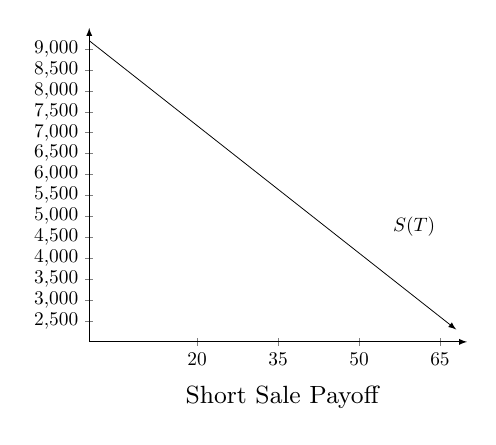
\begin{tikzpicture}[scale=0.7]
	\begin{axis}[
		xmin=0,
		xmax=70,
		xtick={20,35,...,65},
		ymin=2000,
		ymax=9500,
		ytick={2500,3000,...,9000},
		%grid=both,
		axis lines=middle,
		axis line style={->, >=latex},
		x label style={at={(axis description cs:0.86,0.42)},anchor=north},
		xlabel={$S(T)$}]
		%ylabel={payoff},
		%style={font=\tiny}]
		\addplot[black, smooth, domain=0:68, ->, >=latex]{9198-101.51*x};
	\end{axis}
	\node at (3.5, -1) {\small Short Sale Payoff};
\end{tikzpicture}
\hspace{10pt}
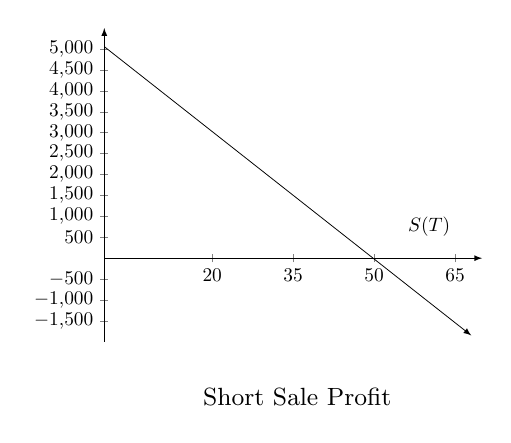
\begin{tikzpicture}[scale=0.7]
	\begin{axis}[
		xmin=0,
		xmax=70,
		xtick={20,35,...,65},
		ymin=-2000,
		ymax=5500,
		ytick={-1500,-1000,...,5000},
		%grid=both,
		axis lines=middle,
		axis line style={->, >=latex},
		x label style={at={(axis description cs:0.86,0.42)},anchor=north},
		xlabel={$S(T)$}]
		%ylabel={profit},
		%style={font=\tiny}]
		\addplot[black, smooth, domain=0:68, ->, >=latex]{5056-101.51*x};
	\end{axis}
	\node at (3.5, -1) {\small Short Sale Profit};
\end{tikzpicture}
\end{center}

These diagrams are meant to illustrate the dangers of short-selling. This is not an activity to enter into lightly. If you find yourself short-selling, you will want to be very knowledgable of the assets you are trading. Alternatively, you may want to try to hedge your position to reduce your loss liability. Derivatives that will be introduced in the next chapter will allow us to protect ourselves from such losses.

Let's return to the discussion of arbitrage. We have a way to determine the price of forward contracts, and we also have ways of replicating that payoff with investments in the underlying asset and cash. Since the payoffs are identical, we can enter into opposite positions that will offset to give us a payoff os zero. This may seem useless; however, when the theoretical price of forward contracts don't match reality we have arbitrage opportunities.

\begin{example}[Forward Contract Arbitrage]
You are in a position to buy a forward contract to purchase 100 shares of XYZ in nine months. The contract costs \$425. The underlying asset price is \$90, and the contract's agreed upon price is \$88. In addition, the dividend rate of the asset is 4\%, and the risk-free rate is 8\%. Determine your arbitrage opportunity.
\end{example}

\begin{solution}
We must start with a computation of the theoretical price of the forward contract:
	\begin{equation*}
	q[S(0)e^{-\delta T}-Ke^{-rT}]=100[90e^{-0.03}-88e^{-0.06}]=446.48
	\end{equation*}
From that, we know that the derivative is underpriced. Since it is underpriced, we should buy it! To ensure that we have no liability in the future, we offset the position by (short) selling $100e^{0.03}$ shares of XYZ today and buying $8800e^{-0.06}$ in risk-free bonds today. The resulting arbitrage opportunity is as follows:
	\begin{itemize}
	\item The forward contract,
	\item a position short of $100e^{-0.03}$ shares in XYZ,
	\item the investment in risk-free bonda of $8800e^{-0.06}$,
	\item and an arbitrage gain of \$21.48
	\end{itemize}
The formal computation for the arbitrage gain would be
	\begin{equation*}
	100e^{-0.03}\cdot 90-8800e^{-0.06}-425=21.48
	\end{equation*}
The reason I didn't do it before displaying the arbitrage gain is that you should know the gain before you write down the portfolio explicitly. It will always be the absolute difference of your two positions. In this case, that is $446.48-425=21.48$.
\end{solution}

\end{document}


